\chapter{Report Body}
%The central part of the report usually consists of three or four chapters detailing the technical work undertaken during the project. {\bf{\textcolor{red}{The structure of these chapters is highly project dependent}}}. They can reflect the chronological development of the project, e.g. design, implementation, experimentation, optimisation, evaluation, etc (although this is not always the best approach). However you choose to structure this part of the report, you should make it clear how you arrived at your chosen approach in preference to other alternatives. In terms of the software that you produce, you should describe and justify the design of your programs at some high level, e.g. using OMT, Z, VDL, etc., and you should document any interesting problems with, or features of, your implementation. Integration and testing are also important to discuss in some cases. You may include fragments of your source code in the main body of the report to illustrate points; the full source code is included in an appendix to your written report.

\section{Algorithms}

\subsection{Lindenmayer Systems}

Hungarian academic Aristid Lindenmayer devised a mathematical model for the reproduction of fungi in 1967.\cite{LINDENMAYER1968300} His model involved a string of symbols, each unique symbol denoting a specific action and/or branch. Essentially, running that initial string, called the \emph{axiom}, through a set of rules (called a \emph{grammar}) gives us an ever-expanding string that is then taken as instructions to draw something from. Lindenmayer Systems, or L-Systems, have since been used in several scenarios beyond its initial purpose of modelling fungi, from trees to fractals. In video games, they are frequently used to aid in the creation of foliage in several environments, as well as buildings and, here, level layouts.

\subsection{Types of Lindenmayer System}

The most basic form of L-System is a \emph{0L}-System, 0 in this case referring to the fact that the grammar is \emph{context-free}.

For this example\cite{lsyspaulbourke}, consider an alphabet $V$, which consists of the following symbols:

\newcommand{\F}{\mbox{F}}

$$ \F, +, - $$

where $\F$ means ``to go forward", and $+$ and $-$ denote turning right or left (respectively) a set number of degrees $\o$.

Take an axiom $\omega$, for example:

$$ \F+\F+\F+\F $$

And a set of rules $P$ which, in this case, is of size 1:

$$ \F \rightarrow \F+\F-\F-\F\F+\F+\F-\F $$

We can represent this \emph{parametric} L-system in the following form:\cite{enwiki:1124510226}

$$ G = (V, \omega, P) $$

To implement $G$ in Godot, we can take each rule and replace each string in accordance to our one rule, using the replace method, like so:

\begin{codeblock}{Simple String Replacement for an L-System with 1 rule}
	string = string.replace(rule["from"], rule["to"]) #Here the rules were stored in dictionaries.
\end{codeblock}

The first 3 iterations of this operation are shown here:

\begin{figure}[H]
	\centering
	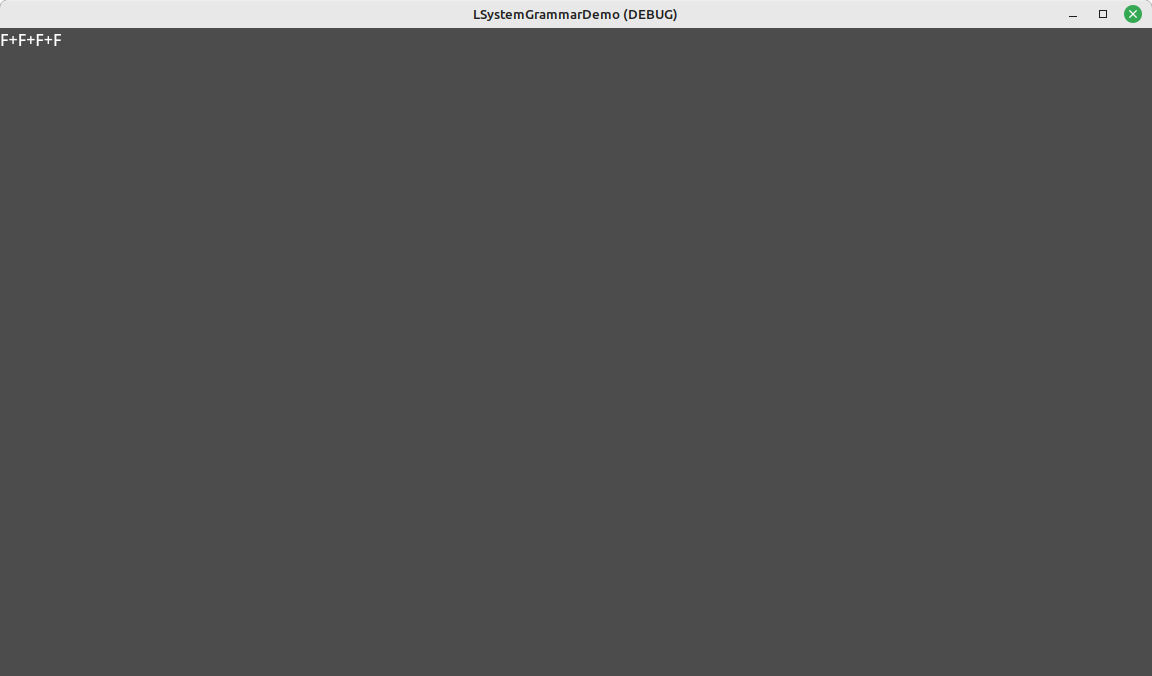
\includegraphics[width=0.5\textwidth]{Images/initial-l-system-iteration-0.png}
	\caption{The axiom of the aforementioned simple L-System with just one rule. String size: 8.\\Source: Own work.}
	\label{fig:lsysiter0}
\end{figure}

\begin{figure}[H]
	\centering
	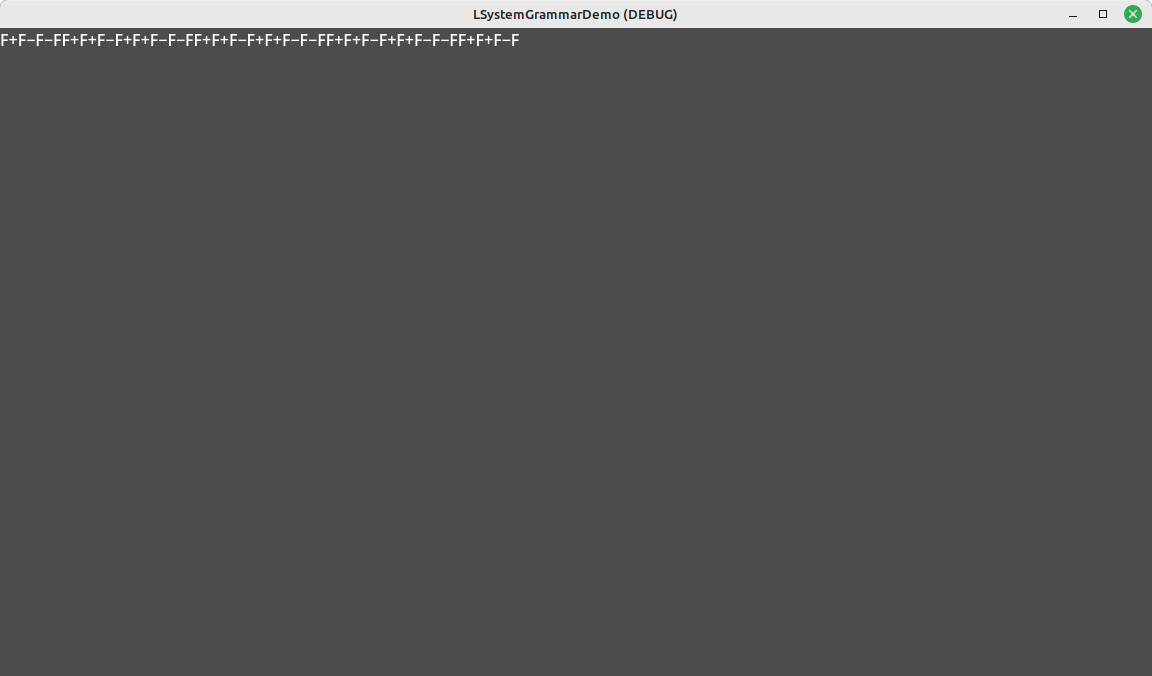
\includegraphics[width=0.5\textwidth]{Images/initial-l-system-iteration-1.png}
	\caption{The first iteration of the aforementioned simple L-System with just one rule. String size: 59.\\Source: Own work.}
	\label{fig:lsysiter1}
\end{figure}

\begin{figure}[H]
	\centering
	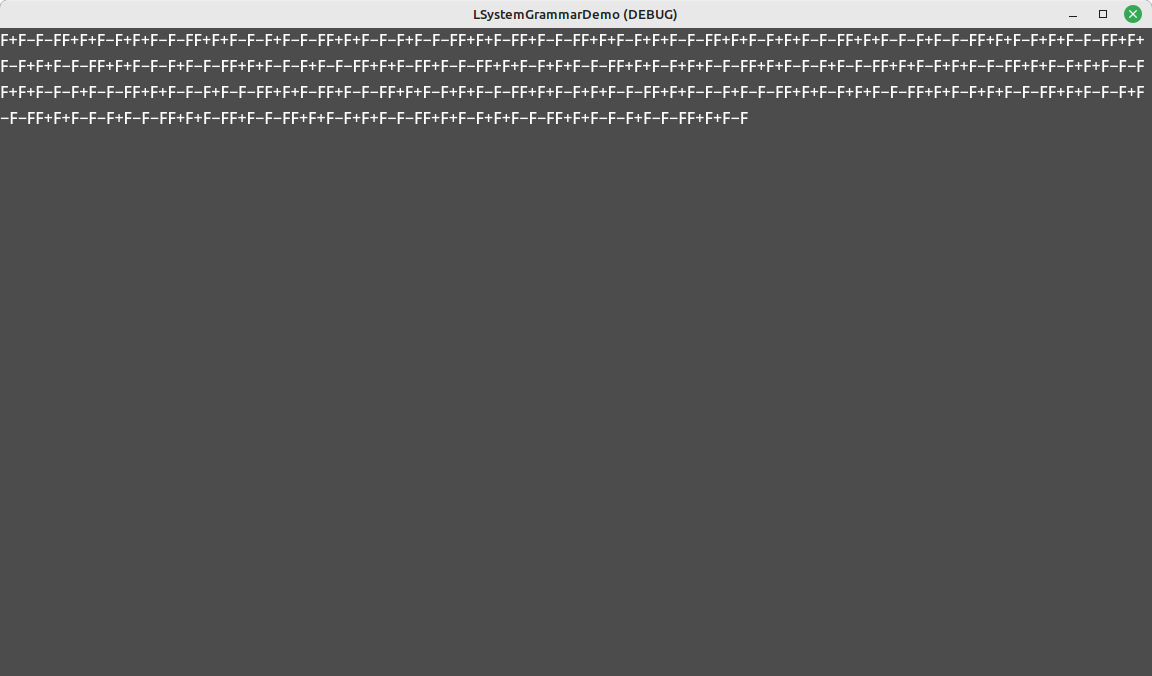
\includegraphics[width=0.5\textwidth]{Images/initial-l-system-iteration-2.png}
	\caption{The second iteration of the aforementioned simple L-System with just one rule. String size: 475.\\Source: Own work.}
	\label{fig:lsysiter2}
\end{figure}

\begin{figure}[H]
	\centering
	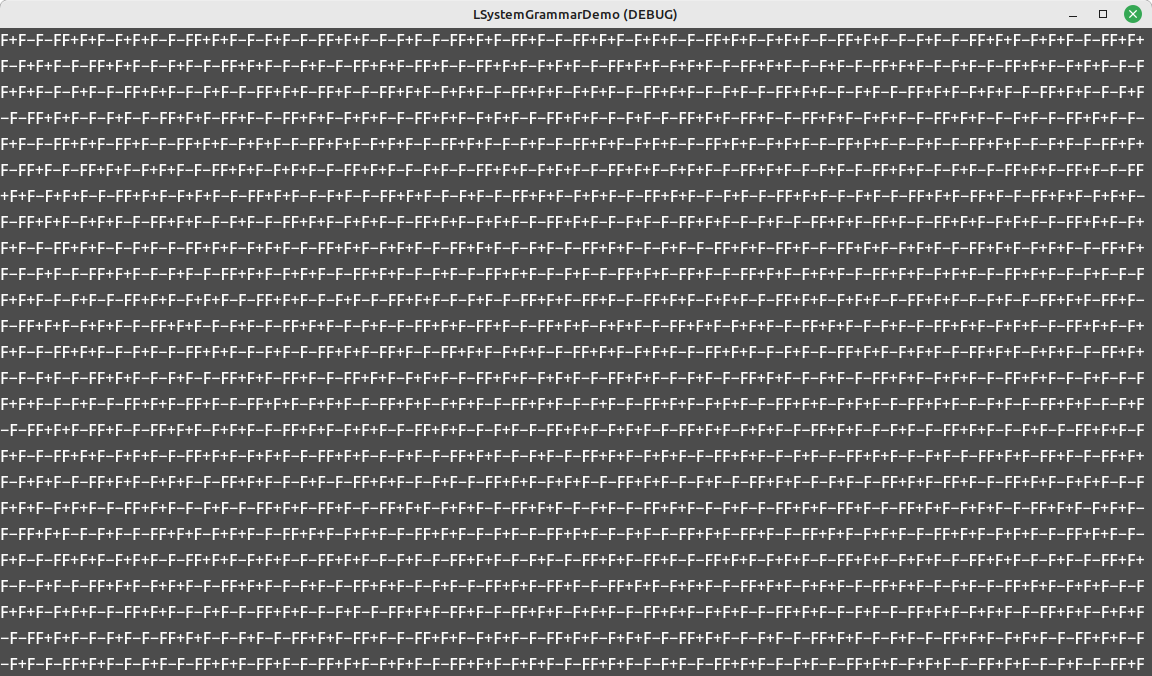
\includegraphics[width=0.5\textwidth]{Images/initial-l-system-iteration-3.png}
	\caption{The third iteration of the aforementioned simple L-System with just one rule. String size: 3803. The string is too large to show in the window, as you can see here.\\Source: Own work.}
	\label{fig:lsysiter3}
\end{figure}

The resulting string can be used to draw a lattice.\cite{lsyspaulbourke} Examples of the above grammar in action are below.

\begin{figure}[H]
    \centering
    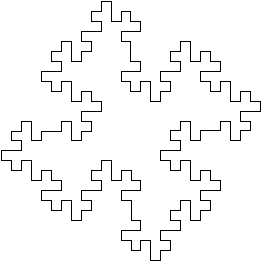
\includegraphics[height=0.25\textheight]{Images/lsys03.png}
    \caption{A lattice generated with the example grammar on a custom-written Classic Mac OS application specifically written for working with L-Systems.\cite{lsyspaulbourke}}
    \label{fig:lattice1}
\end{figure}

\begin{figure}[H]
    \centering
    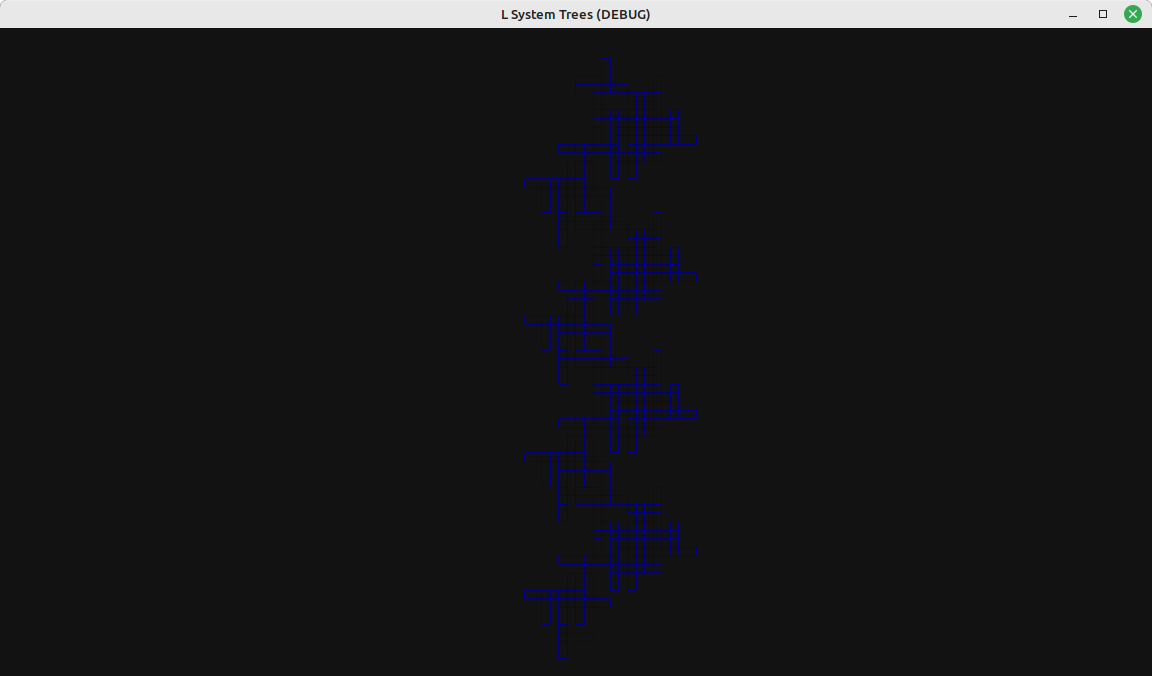
\includegraphics[width=0.75\textwidth]{Images/gd4lattice.png}
    \caption{A lattice generated with the example grammar on a Godot project for drawing from L-Systems. Source: Initial project written by YouTuber Codat, and converted to Godot 4 (with the addition of the lattice grammar) by me.}
    \label{fig:my_label}
\end{figure}

\subsection{Voronoi Cells}

Voronoi cells work by taking a map of points, and randomly selecting a group of points. Within that selected group, cells are formed by calculating, in each point of the grid, the closest of the selected points to it. Distances between points can be calculated with either the Euclidean or Manhattan distance. 

\subsection{Poisson Disk Sampling}

Poisson disk distributions are an easy way to randomly scatter objects across a field. It's commonly used for tree placement. It takes a 

\subsection{Simplex Noise}

Kenneth Perlin designed a type of noise named after himself (Perlin Noise), in which each pixel of noise is affected by its surroundings. 

\section{Implementations}